\documentclass[dvipdfmx,10pt,notheor]{beamer}
\mode<presentation> 
\usepackage[orientation=portrait, %縦書きの場合は portrait 横書きの場合は landscape
            size=a0,              %a0,a1,a2,a3,a4からサイズを選択
            scale=1.4,            %フォントサイズ
            debug                 %不明（直訳:デバッグ）
            ]{beamerposter}
\usepackage[japanese]{babel}      %日本語で作るとき必須
%==========================================================================================
%==========================================================================================
%%% パッケージを追加するところ
\usepackage[utf8]{inputenc}

%% 字体/記号/ルビ/その他 関係のパッケージ
\usepackage{amsmath,amssymb}
\usepackage{mathtools}
\usepackage{amsfonts}
\usepackage{mathrsfs}              %さまざまな字体追加
\usepackage{latexsym}              %数式で使える記号を増やす
\usepackage{centernot}             %not記号をつける
\usepackage[dvipsnames]{xcolor}    % 文字に好きな色をつける

%% 図の挿入関係のパッケージ
\usepackage{graphicx}              %図の挿入
\usepackage{float}                 %図の位置指定
\usepackage{here}                  %好きな位置に図を配置
\usepackage{caption}               %図・表 (Figure & Table) キャプションのカスタマイズ
\usepackage{array,booktabs}        %表組み

%% ボックス系のパッケージ
\usepackage{tcolorbox}             %beamerで好きな色のboxをつくる
\usepackage{ascmac}                %screen環境,itembox環境,shaddbox環境の追加

%% beamerのhyperref環境
\usepackage{pxjahyper}             % hyperrefとセットのパッケージ/PDF化の際に文字化けを防ぐ
\hypersetup{
  colorlinks=false,
  pdfborder={0 0 1},
  citebordercolor=green,
  linkbordercolor=red,
  urlbordercolor=cyan,
  hidelinks
}
% 参考(beamer)：https://charmie11.hatenablog.com/entry/2021/10/07/110625
% 参考（一般）：https://mathlandscape.com/latex-hyperref/

\usepackage{kantlipsum}            % ダミーテキストの生成
%==========================================================================================
%==========================================================================================
%%% beamerの基本設定

\usetheme{Berlin}                              % beamerのテーマの選択
\usecolortheme{orchid}                         % カラーテーマの選択
\useinnertheme{circles}                        % フレーム内のテーマの選択
\useoutertheme{default}                        % フレーム外のテーマの選択
\usefonttheme{professionalfonts}               % フォントファミリー設定
% \usefonttheme[onlymath]{serif}                 % 英文をサンセリフ体に
\renewcommand{\kanjifamilydefault}{\gtdefault} % 既定をゴシック体に

\setbeamertemplate{footline}[frame number]     % footline       非表示（最下段から一番目のみ消去）
\setbeamertemplate{navigation symbols}{}       % ナビゲーションバー非表示（最下段から二番目のみ消去）

%% ロゴが右下に出ないようにする
\defbeamertemplate*{sidebar right}{sidebar theme}
    {%
    \vfill%
    \llap{\usebeamertemplate***{navigation symbols}\hskip0.1cm}%
    \vskip2pt
    }

%% boxの設定（丸み/影なし）
\setbeamertemplate{blocks}[rounded][shadow=false]

%===========================================================================================
%===========================================================================================
%%% 色の設定

%% テーマカラーの設定（デフォルトとは青色）
\setbeamercolor{structure}{fg=cyan!90!black!}             %メインカラーの色変更

%% 背景の色の変更（デフォルトとは白色）
\setbeamercolor{background canvas}{bg=yellow!20}

%% box系の色設定
\setbeamercolor{block title}{fg=white, bg=blue!40!white} %ノーマルブロックの色変更
\setbeamercolor{block body}{fg=black, bg=red!10!white}  %ノーマルブロックの色変更
\setbeamercolor{alerted text}{fg=red!50}                   %アラートボックスの色変更
\setbeamercolor{example text}{fg=green}                   %exampleボックスの色変更

%===========================================================================================
%===========================================================================================
%%% mybox環境の作成
\newtcolorbox{mybox}[1]
{
    title=#1, 
    toptitle=2mm, bottomtitle=2mm, 
    colframe=structure,boxrule=5pt,
    coltitle=white, colbacktitle=structure,
    colback=white, fonttitle=\bfseries\Large,
    top=5mm, bottom=5mm, left=5mm, right=5mm, %内部余白調整
    enlarge top by=1mm, enlarge bottom by=1mm, %外部余白調整
}

%%% head(\maketitle)環境の作成・設定
\setbeamertemplate{headline}{
    \structure{
        \vskip3ex
        \begin{center}
            \rule{0.98\linewidth}{4mm}
        \end{center}
        \vskip3ex
        \begin{columns}[T]
             \begin{column}{.67\linewidth}
                \begin{center}
                    \usebeamercolor{title in headline}{\textbf{\LARGE{\inserttitle}}\\[2.5ex]}
                    \usebeamercolor{author in headline}{\large{\insertauthor}\\[1.2ex]}
                    \usebeamercolor{institute in headline}{\large{\insertinstitute}}
                \end{center}
            \end{column}
            \begin{column}{.31\linewidth}
                \begin{center}
                    \insertlogo
                \end{center}
            \end{column}
        \end{columns}
        \vskip3ex
        \begin{center}
            \rule{0.98\linewidth}{4mm}
        \end{center}
    }
}

%%% foot環境の作成・設定
\setbeamertemplate{footline}{
    \begin{center}
        \structure{
            \rule{0.98\linewidth}{2mm}
            \vskip4ex
            \begin{columns}[T]
                \begin{column}{0.90\paperwidth}
                    \begin{flushright}
                        \usebeamercolor{conference in headline}{\large{\foot}}
                    \end{flushright}
                \end{column}
            \end{columns}
            \vskip3ex
        }
    \end{center}
}

%%% itemize環境の作成
\setbeamertemplate{itemize item}{\small\raise0.5pt\hbox{$\bullet$}}
\setbeamertemplate{itemize subitem}{\tiny\raise1.5pt\hbox{$\blacktriangleright$}}
\setbeamertemplate{itemize subsubitem}{\tiny\raise1.5pt\hbox{$\bigstar$}}

%%% enumerate環境の作成
\setbeamertemplate{enumerate item}%{\small\raise0.5pt\hbox{$\bullet$}}


%=======================================================================================
%=======================================================================================
%%% 定理環境の作成，関連コマンド
\usepackage{amsthm} %定理環境のパッケージ
\theoremstyle{definition}
\numberwithin{equation}{section}      %数式番号
\newtheorem{dfn}{定義}[section]
\newtheorem{thm}[dfn]{定理}
\newtheorem{prop}[dfn]{命題}
\renewcommand{\proofname}{\textbf{証明}}     %証明の名前の変更



%=======================================================================================
%=======================================================================================
%%% maketitleとfootlineの入力欄
\title{タイトル}
\author{氏名}
\institute{所属}
\newcommand{\foot}{研究集会\quad (場所，日付)}
\logo{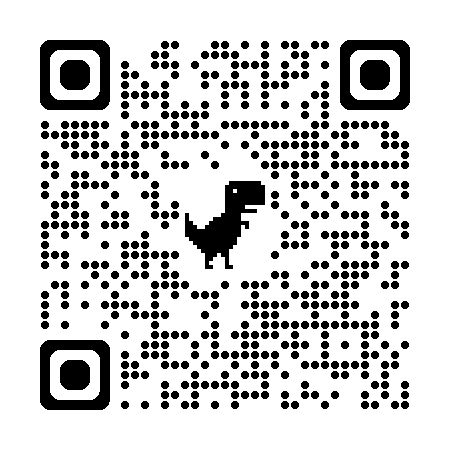
\includegraphics[height=7.5cm]{HPhoshino.png}}   % スライドの右上に画像を表示させる
%=======================================================================================
%=======================================================================================

\begin{document}
\begin{frame}{}
%%%%%%%%%%%%%%%%%%%%%%%%%%%%%%%%%%%%%%%%%%%%%%%%%%%%%%%%%%%%%%%%%%%%%%%%%%%%%%%%%%%%%%%%%%%%%
%%%%%%%%%%%%%%%%%%%%%%%%%%%%%%%%%%%%%%%%%%%%%%%%%%%%%%%%%%%%%%%%%%%%%%%%%%%%%%%%%%%%%%%%%%%%%
\vfill


\begin{columns}[T]
\begin{column}{.98\linewidth}
\begin{mybox}{1. item環境・enumerate環境のテスト}
\begin{minipage}[t]{0.45\textwidth}
    \vspace{0pt}
    これは{\LARGE{\color{red} 『ダミーテキスト』}}です．\\
    \kant[1]
\end{minipage}
\hfill
\begin{minipage}[t]{0.45\textwidth}
    \vspace{0pt}
    item環境のテスト
    \begin{itemize}
        \item a
        \item b
        \item c
    \end{itemize}
    enumerate環境のテスト
    \begin{enumerate}
        \item [] A
        \item [$( \mathrm{i} )$] B
        \item [$(2)$] C
    \end{enumerate}
\end{minipage}
\end{mybox}
\end{column}
\end{columns}


\vfill


\begin{columns}[T]
\begin{column}{.48\linewidth}
\begin{mybox}{2. tcolorboxのテスト}

\begin{tcolorbox}[left=1mm,
                  colframe=blue,
                  colback=blue!5!white,
                  colbacktitle=blue!70!black,
                  coltitle=white, fonttitle=\bfseries,
                  title=ヘッダー]
    本文
\end{tcolorbox}

\begin{tcolorbox}[left=1mm,
                  colframe=red,
                  colback=red!10!white,
                  colbacktitle=red,
                  coltitle=white, fonttitle=\bfseries,
                  title=定義・定理・命題・事実・問題設定など]
    色は好きに設定可能
\end{tcolorbox}
\end{mybox}
\vfill
\begin{mybox}{3. tcolorboxのテスト}
\begin{tcolorbox}[left=1mm,
                  colframe=orange,
                  colback=orange!10!white,
                  colbacktitle=orange!40!white,
                  coltitle=black, fonttitle=\bfseries,
                  title=定義]
    本文
\end{tcolorbox}
\begin{tcolorbox}[left=1mm,
                  colframe=magenta,
                  colback=magenta!0!white,
                  colbacktitle=magenta!40!white,
                  coltitle=black, fonttitle=\bfseries,
                  title=Main Theorem]  
    本文
\end{tcolorbox}
\begin{tcolorbox}[left=1mm,
                  colframe=cyan,
                  colback=cyan!10!white,
                  colbacktitle=cyan!40!white,
                  coltitle=black, fonttitle=\bfseries,
                  title=定理]
\end{tcolorbox}
\begin{tcolorbox}[left=1mm,
                  colframe=green,
                  colback=green!10!white,
                  colbacktitle=green!40!white,
                  coltitle=black, fonttitle=\bfseries,
                  title=例]  
    本文
\end{tcolorbox}
\begin{tcolorbox}[left=1mm,
                  colframe=lightgray,
                  colback=lightgray!10!white,
                  colbacktitle=lightgray!40!white,
                  coltitle=black, fonttitle=\bfseries,
                  title=Fact]
    本文
\end{tcolorbox}
\end{mybox}
\end{column}


\begin{column}{.48\linewidth}
\begin{mybox}{4. box類のテスト}
    \begin{block}{blockの表示}
        色は好きに設定可能
    \end{block}
    \begin{alertblock}{alertblockの表示}
        色は好きに設定可能
    \end{alertblock}
    \begin{exampleblock}{exampleblockの表示}
        色は好きに設定可能
    \end{exampleblock}
\end{mybox}
\vfill
\begin{mybox}{5. 定理環境のテスト}
    \begin{thm}
        メインカラーに依存
    \end{thm}
    \begin{prop}
        メインカラーに依存
    \end{prop}
    \begin{proof}
        begin\{proof\}の環境\\
        メインカラーに依存
    \end{proof}
\end{mybox}
\end{column}
\end{columns}


\vfill


\begin{columns}[T]
\begin{column}{.98\linewidth}
\begin{mybox}{6. 配置のテスト}
    
\end{mybox}
\end{column}
\end{columns}


%\vfill


\begin{columns}[T]
\begin{column}{.48\linewidth}
\begin{mybox}{7. 配置のテスト}
\end{mybox}
\end{column}
\begin{column}{.48\linewidth}
\begin{mybox}{8. 配置のテスト}
\end{mybox}
\end{column}
\end{columns}


\vfill


\begin{columns}[T]
\begin{column}{.98\linewidth}
% \begin{mybox}{.参考文献}
    参考文献
    \footnotesize                % サイズの縮小
    \beamertemplatetextbibitems % 番号を表示
    \begin{thebibliography}{99}
        \bibitem{ttss} 
        著者，
        タイトル，
        出版社，
        出版年．
    \end{thebibliography}           
% \end{mybox}
\end{column}
\end{columns}


\vfill
%%%%%%%%%%%%%%%%%%%%%%%%%%%%%%%%%%%%%%%%%%%%%%%%%%%%%%%%%%%%%%%%%%%%%%%%%%%%%%%%%%%%%%%%%%%%%
%%%%%%%%%%%%%%%%%%%%%%%%%%%%%%%%%%%%%%%%%%%%%%%%%%%%%%%%%%%%%%%%%%%%%%%%%%%%%%%%%%%%%%%%%%%%%
\end{frame}
\end{document}